\newpage
\section{Ranking}
In this section, the estimators from the previous section will be used to give an estimated ranking for best strategies that could be used on an unseen dataset, to answer research question 3: \textit{Is it possible to generate a ranking of tools according to their performance on unseen datasets?}
~\\~\\In the following section, the results will be based on the ranking generated by the F1-score estimators from the previous section. Only the NDCG based on the F1-score will be used to give the qualitative evaluation. For each experiment, the best strategy ranking estimator (either the combined F1-estimator or direct F1-estimator) will be shown and evaluated. In the last section, overall performance across all the rankings will be compared to the baseline method to evaluate the results quantitatively.

\subsection{Best tool ranking}
For finding the best tool, the strategy ranking with only a single configuration per tool was created. Like stated in \autoref{sec:toolranking}, there were two ways of scoring this ranking:

\subsubsection{Strategy-based scoring}
The first way of scoring was strategy-based scoring. For this experiment the direct F1 estimator was the best performing underlying estimator for generating the ranking. In figure \autoref{fig:ndcg_per_strategy}, the NDCG scores are shown with relevance according to the suggested specific strategy.

As shown in the figure, for two out of the fourteen datasets, the score is less than half the top score (1). This implies that, for those datasets, the suggested strategy ranking placed less performing strategies higher at the top and/or gave less performing configurations of a tool priority over a better configuration. 

\begin{figure}[H]
    \centering
    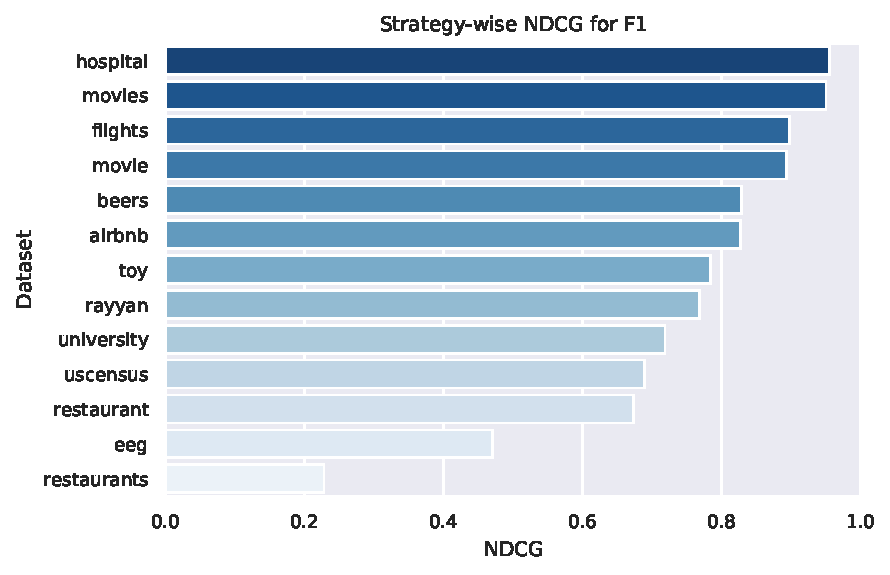
\includegraphics[width=0.9\textwidth]{thesis/Figures/RQ3/15_ranking_ndcg_F1_strategy_wise.pdf}
    \caption{NDCG per dataset for strategy ranking of the direct F1 estimator}
    \label{fig:ndcg_per_strategy}
\end{figure}


\subsubsection{Tool-based scoring}
The other way of scoring, tool-wise scoring, was were the NDCG scores calculated with relevance according to the highest scoring strategy of that tool. In this scoring way, the configurations of the ranking are disregarded and there is only a focus on the ordering of tools. The direct F1-estimator performed slightly (+0.01 increase in NDCG) better than the combined F1-estimator. The results can be seen in \autoref{fig:ndcg_per_tool}. 
The resulting tool-wise NDCG scores are 0.211 (0.956 vs 0.745) higher than the NDCG scores for the strategy-wise scoring. This means that the recommended strategy ranking is better at finding the right tool, but not necessarily selects the best single configuration for that tool. The ordering for each dataset is nearly perfect, except for \verb|Toy| (really small dataset) and \verb|Restaurants| (where the highest F1 score was 0.01, so an outlier among the datasets). 

\begin{figure}[H]
    \centering
    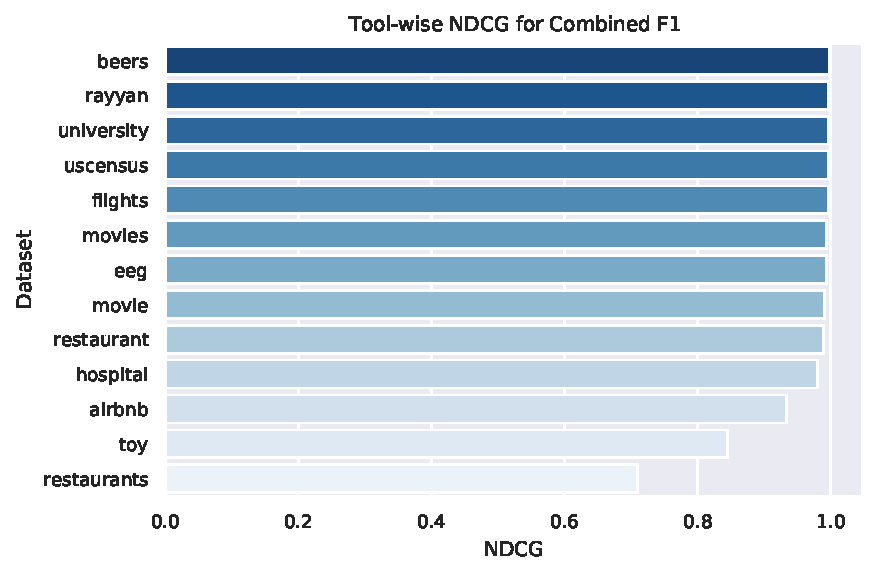
\includegraphics[width=0.9\textwidth]{thesis/Figures/RQ3/15_ranking_ndcg_combined_f1_tool_wise.pdf}
    \caption{NDCG per dataset for tool ranking of the direct F1 estimator}
    \label{fig:ndcg_per_tool}
\end{figure}


\subsection{Best configuration ranking}
Following the results from \autoref{fig:ndcg_per_tool}, where it has been shown that a good ranking of tools can be made, the next section will discuss configuration ranking for a single tool. The two error detection tools that will be covered are Raha and dBoost. The two tools are the best performing tools overall and have both have numerous configuration options, making it worthwhile to generate a configuration ranking.

\subsubsection{Raha} 
For estimating ranking of the best configurations for Raha, the direct F1 estimator performed best.
With a mean NDCG of 0.824, the configuration ranking for Raha is really promising. For most of the datasets, the ranking is near-optimal. As shown in \autoref{fig:ndcg_per_config_Raha}, only for two datasets, the score is below half optimal. This means that for those datasets, wrong suggestions will be made for the configurations to use. For the majority of datasets, the ranking system is able to output the configuration in a ordering where the top suggestions also correspond with high performance results from the empirical study. For the worst-performing dataset, \verb|Restaurants|, the F1-score for Raha was 0.00 for the empirical study. This results in no possible best ranking.

\begin{figure}[H]
    \centering
    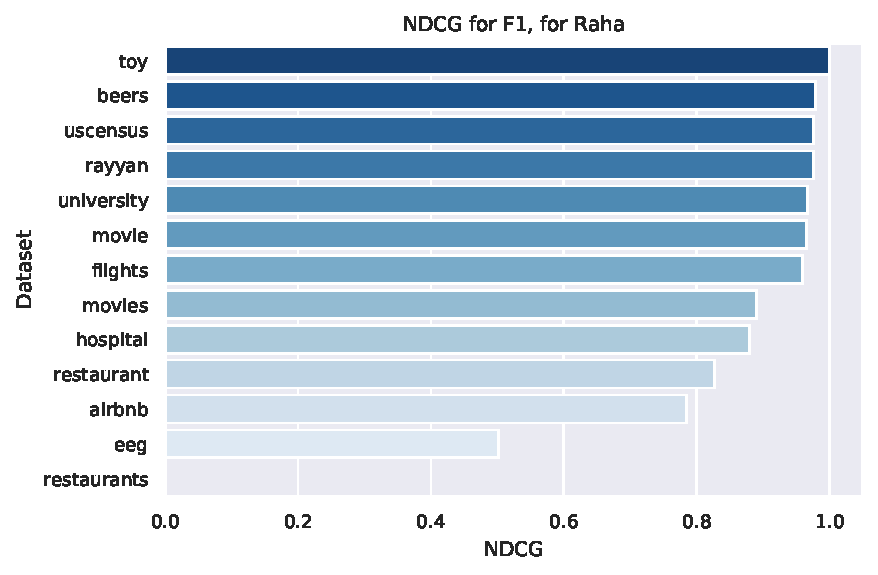
\includegraphics[width=0.9\textwidth]{thesis/Figures/RQ3/15_f1_profiler_NDCG_Raha.pdf}
    \caption{NDCG per dataset for configuration ranking of the direct F1 estimator for Raha}
    \label{fig:ndcg_per_config_Raha}
\end{figure}

\subsubsection{dBoost} 
For estimating ranking of the best configurations for dBoost, the combined F1 estimator performed best.
With a mean NDCG of 0.572, the configuration ranking for dBoost is worse than the generated configuration rankings of Raha. A score of 0.572 corresponds to an just above decent ranking on average. This means that, for some datasets, it is able to output correct rankings, but for others, it can completely not. With dBoost, the difference between the best and worst-performing strategies is more significant than the difference between Raha strategies. 

Also, certain dBoost configurations are locally non-sensitive, meaning that small changes in the configurations do not have a great impact on the results. These locally insensitive configurations can be grouped together based on more influential parameters. This also implies that, if an estimate for a configuration is given, the configuration in the same group will also have similar estimates.  If one of these estimates is an over-estimation, multiple estimations will be too high, resulting in a worse ranking. Future improvements of the ranking system could include protection against these grouped estimations causing worse results.

\begin{figure}[H]
    \centering
    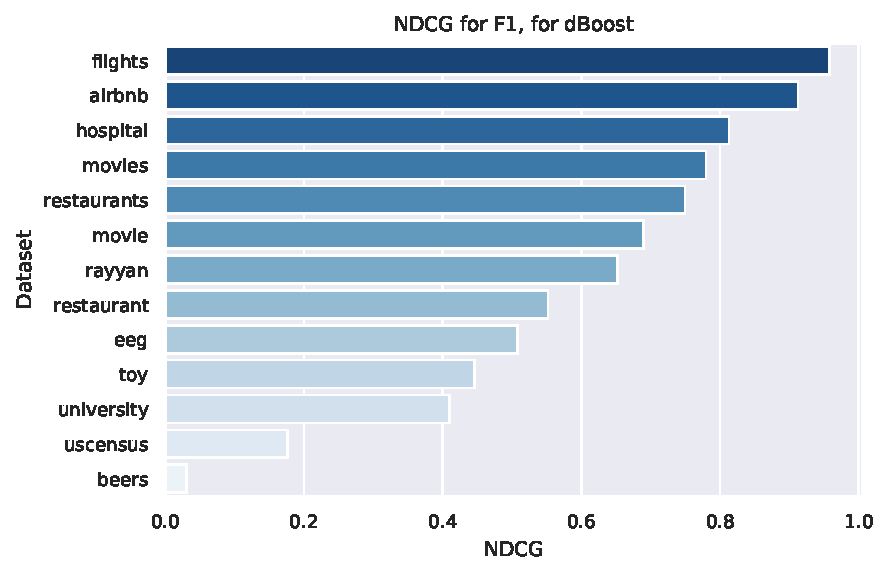
\includegraphics[width=0.8\textwidth]{thesis/Figures/RQ3/15_combined_profiler_NDCG_dBoost.pdf}
    \caption{NDCG per dataset for configuration ranking of the combined F1 estimator for dBoost}
    \label{fig:ndcg_per_config_dBoost}
\end{figure}


\subsection{Evaluation}
\label{subsec:results_ranking_evaluation}
In the sections above, the different NDCG values for the experiment per dataset have been shown. Below, a further evaluation will follow.
% \paragraph{Qualitative} The NDCG values per dataset for each experiment will be sorted and plotted for comparison. The focus of the qualitative analysis will be that of the ordering and general relative results between datasets in one experiment. Preferably, NDCG values per dataset are similarly high, without many lower outliers. If there is a cluster of lower NDCG values, the ranking will be deemed meaningless.
Qualitatively, the ranking scores are promising. For the tool ranking with tool-wise NDCG scoring, the ranking system was able to generate high-quality output, without any lower outliers. When looking at the strategy-wise scored rankings (where the suggested configuration is also taken into account), the NDCG is of course "discounted", due to the stricter scoring criteria. Still, only two datasets have an NDCG below 0.5. For all other datasets, more than decent rankings have been returned, so there are no large clusters of low outliers in terms of ranking results. The same holds for the configuration ranking for Raha. With the \verb|Restaurants| dataset, it was not possible to generate any good rankings, due to the 0 F1-score, and for the \verb|EEG| dataset, it was close to half optimal. For the other datasets, the ranking system was capable of generating a well ordered ranking with respect to optimal configurations for Raha. Lastly, for the configuration suggestion ranking of dBoost, the NDCG values were the lowest. It contained more lower-ranking results, showing that is was harder to estimate the right order of configurations. 

% \paragraph{Quantitative} Similar to \autoref{sec:performanceprediction}, the results of the experiments will be compared to a baseline method. This baseline method estimates performance as described in \autoref{subsec:evaluation_performanceprediction}. From these baseline estimation, rankings of the same structure as in the experiments will be created and scored with NDCG. While the focus lies on the F1-score for this section, a comparison of mean NDCG for all datasets will be compared for precision based ranking, recall based ranking and F1 based ranking, both directly estimated and combinedly estimated (recall + precision estimation to calculate the estimated F1).

Quantitatively, a comparison between the proposed strategy ranking system with performance estimators based on the dataset profiles and the baseline method will be discussed below. Similarly to the evaluation of the previous section and research question (\autoref{subsec:results_prediction_evaluation}), there will be looked at a quantitative improvement over the scores between both systems. For all four experiments described in the results and figures above, this comparison will be made. 
First, the mean strategy-wise NDCG tool ranking results will be compared, as shown in \autoref{tab:mean_strategy_wise_NDCG_comparison}. Overall, for all the ranking/estimator types (Precision, Recall, F1 and Combined F1), the proposed method improves over the baseline. The scores for the precision and recall are also included. It is a possibility to investigate these more in future research. Especially the results for estimated precision ranking could be used in automated error detection workflows. 

\begin{table}[H]
\centering
\begin{tabular}{lrlr}
\toprule
{} &  Baseline &  Estimator &   \\
Metric          & Mean NDCG  &  Mean NDCG  &       Improvement       \\
\midrule
Combined F1 &          0.540 &  \textbf{0.654} &        0.114 \\
F1          &          0.690 &  \textbf{0.745} &        0.055 \\
Precision   &          0.495 &  \textbf{0.571} &        0.077 \\
Recall      &          0.885 &  \textbf{0.905} &        0.020 \\
\bottomrule
\end{tabular}
\caption{Mean strategy-wise NDCG comparison for tool ranking (best scores in bold)}
\label{tab:mean_strategy_wise_NDCG_comparison}
\end{table}


For the other 3 experiments (tool-wise NDCG tool ranking, Raha configuration ranking \& dBoost ranking), the same results are shown in \autoref{app:ranking}. For the tool-wise scored tool ranking results, the baseline and proposed system score close to equal on all estimation tasks. Also, the mean NDCG of these rankings are close to 1. This implies that for tool ranking and looking only at the tools for scoring (not at the suggested configurations), simply taking the best previous tool is enough to generate good rankings and cannot be improved much further. 
For the configuration ranking for Raha, the proposed system scores better than the baseline on all metrics. 
For dBoost, this not the case. The proposed system performs best on estimating the F1 score (using the combined estimator) and estimating the precision. However, the baseline performs better in estimating recall. However, the emphasis for ranking lies more on F1 and precision, as recall by itself is not meaningful (selecting all values as erroneous will give 1.00 as recall), so combining the improvement over the baseline of the F1 rankings and precision rankings, still shows the potential of the proposed ranking system.

The proposed ranking system based on the performance estimators has shown to be promising both qualitatively and quantitatively among the majority of datasets. The proposed system outperformed the set baseline and was able to create valuable rankings for different tasks, namely tool ranking and configuration ranking for a specific tool. This has shown that it is possible to generate a ranking of tools according to their performance on unseen datasets.

% The main comparison to answer if it possible to generate a ranking of tools according to their performance on unseen datasets, will be to see if there is an increase in the mean NDCG for all experiments from the proposed estimator compared to the baseline, described in the paragraph above. If there is no increase in NDCG, the estimator will be deemed not suitable for estimated strategy ranking. 